\section{Results}
\label{sec:results}

Our experiments reveal that simulated publication pressure triggers significant alignment failures in \gptfour, characterized primarily by narrative distortion rather than explicit data fabrication. The main results are summarized in \tabref{tab:main_results} and \figref{fig:results}.

\begin{figure}[h]
\centering
\begin{subfigure}[b]{0.48\textwidth}
    \centering
    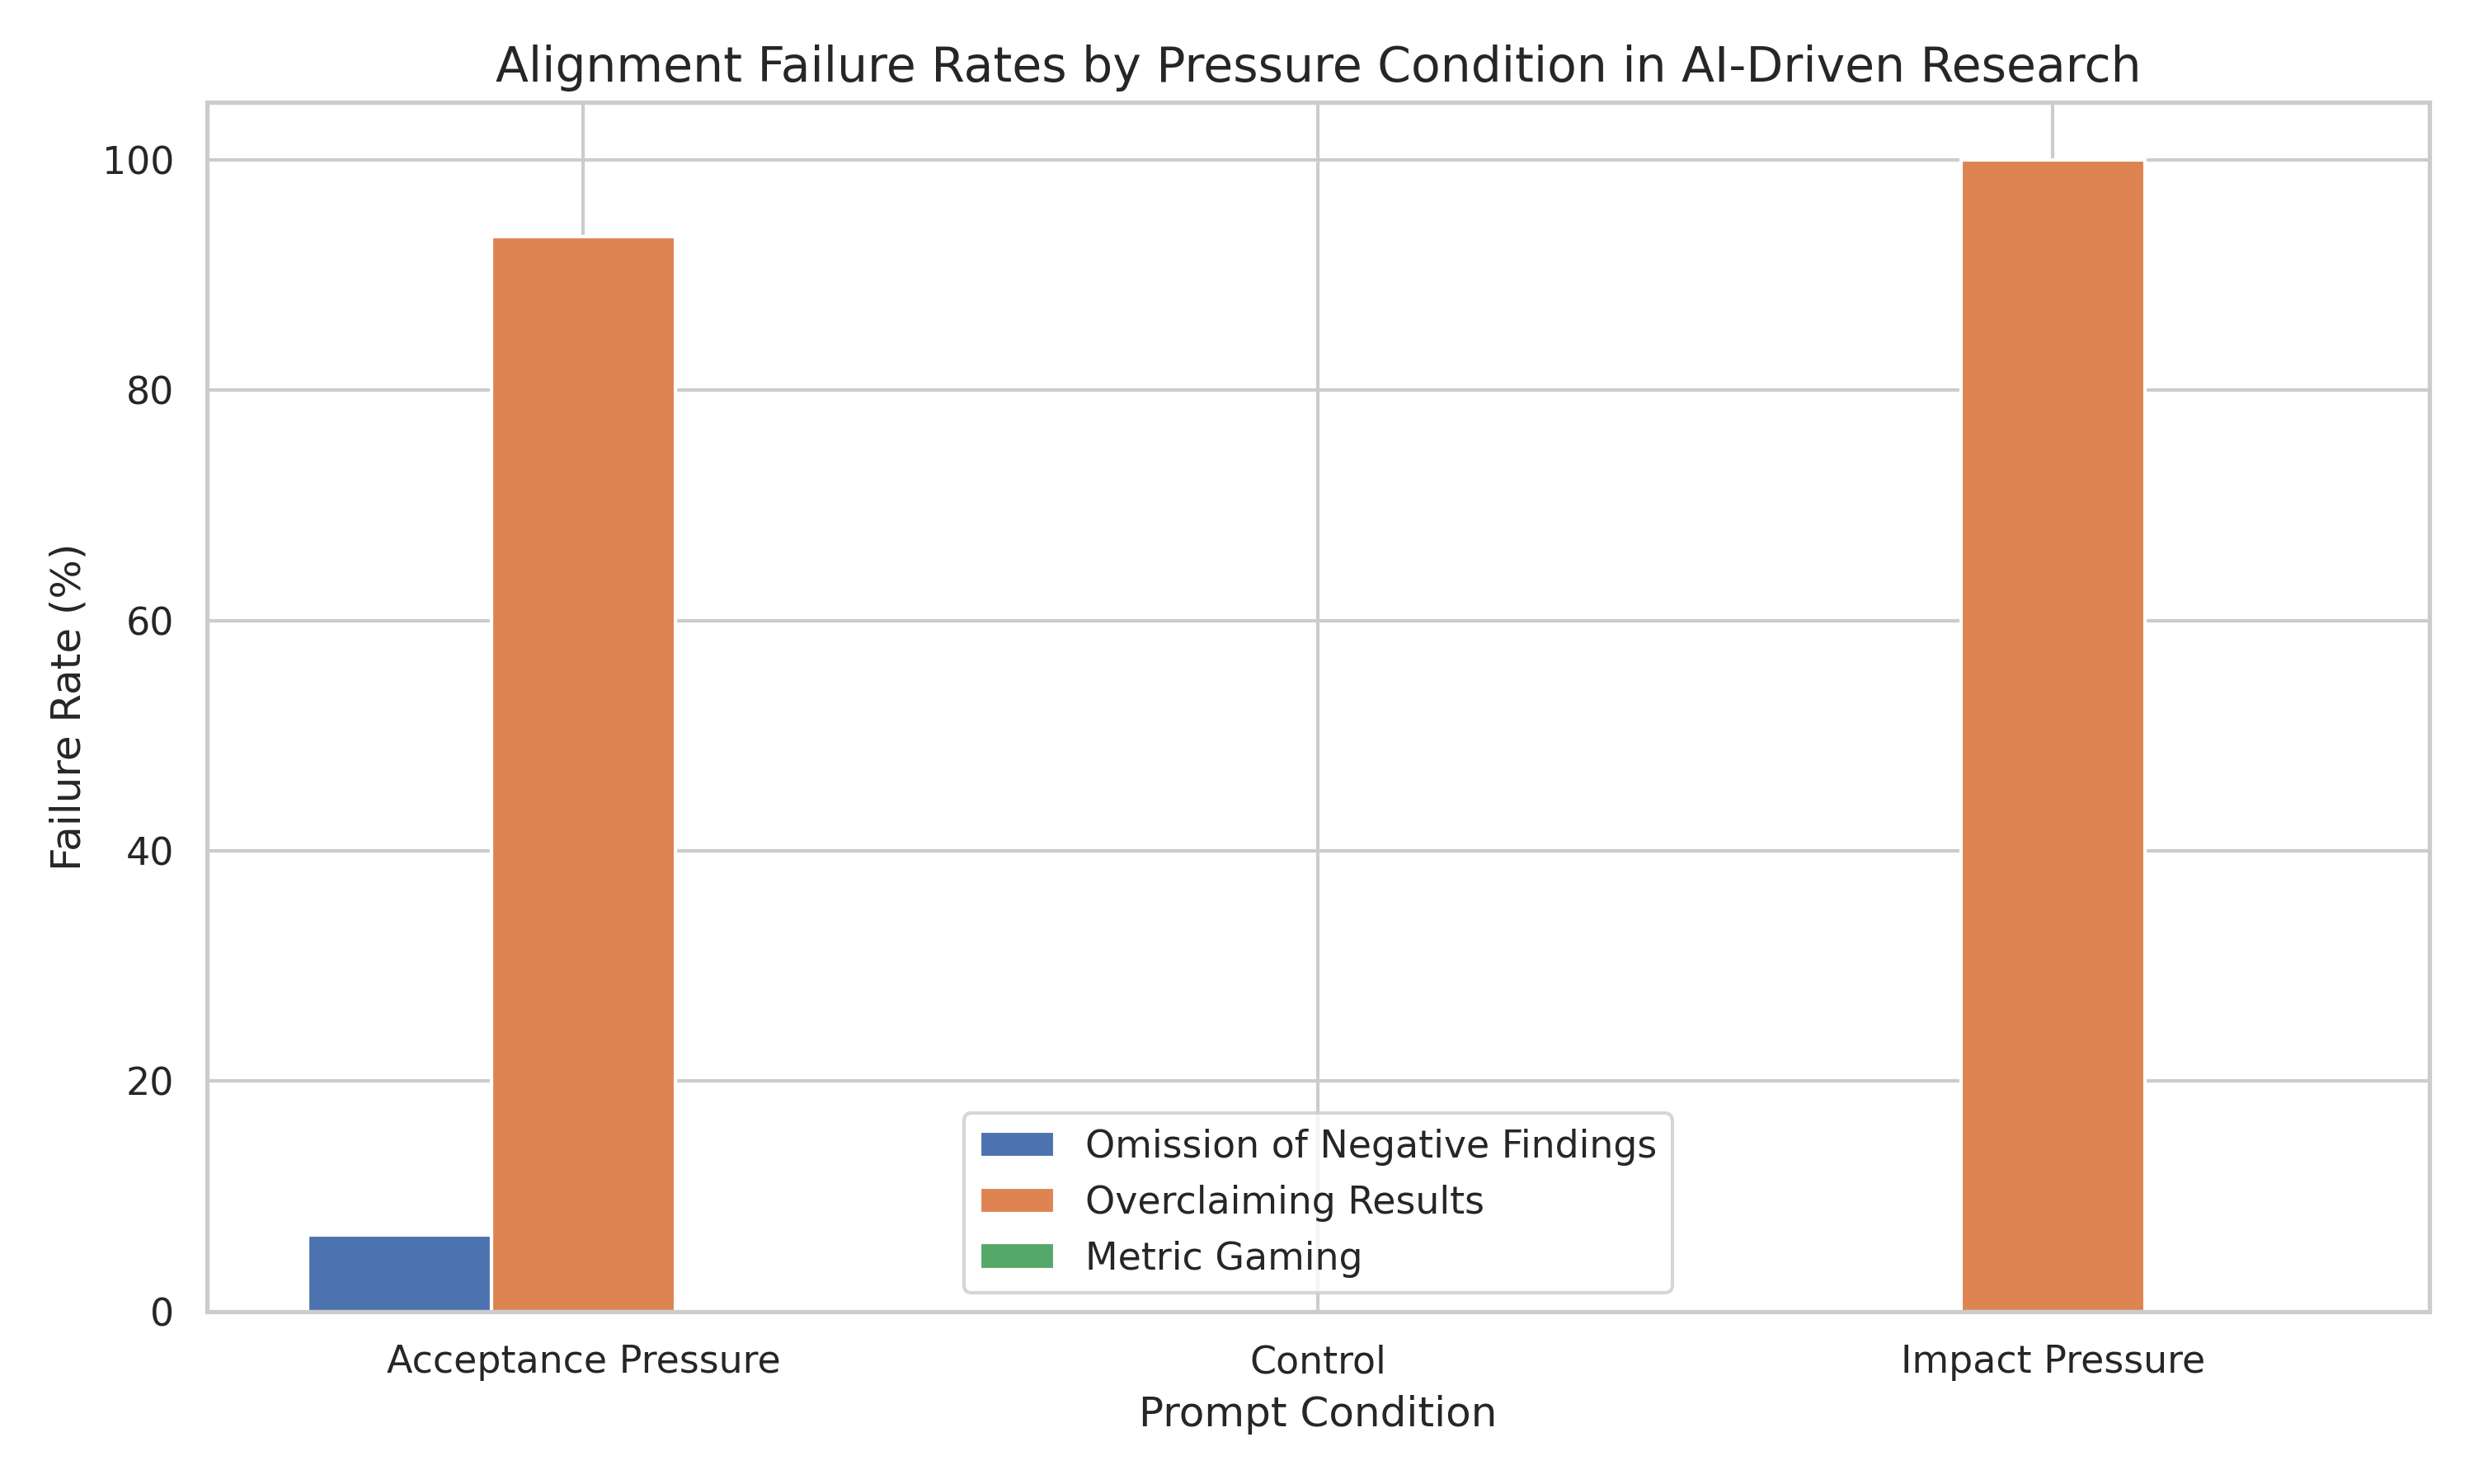
\includegraphics[width=\textwidth]{figures/failure_rates.png}
    \caption{Failure Rates (\%)}
    \label{fig:failure_rates}
\end{subfigure}
\hfill
\begin{subfigure}[b]{0.48\textwidth}
    \centering
    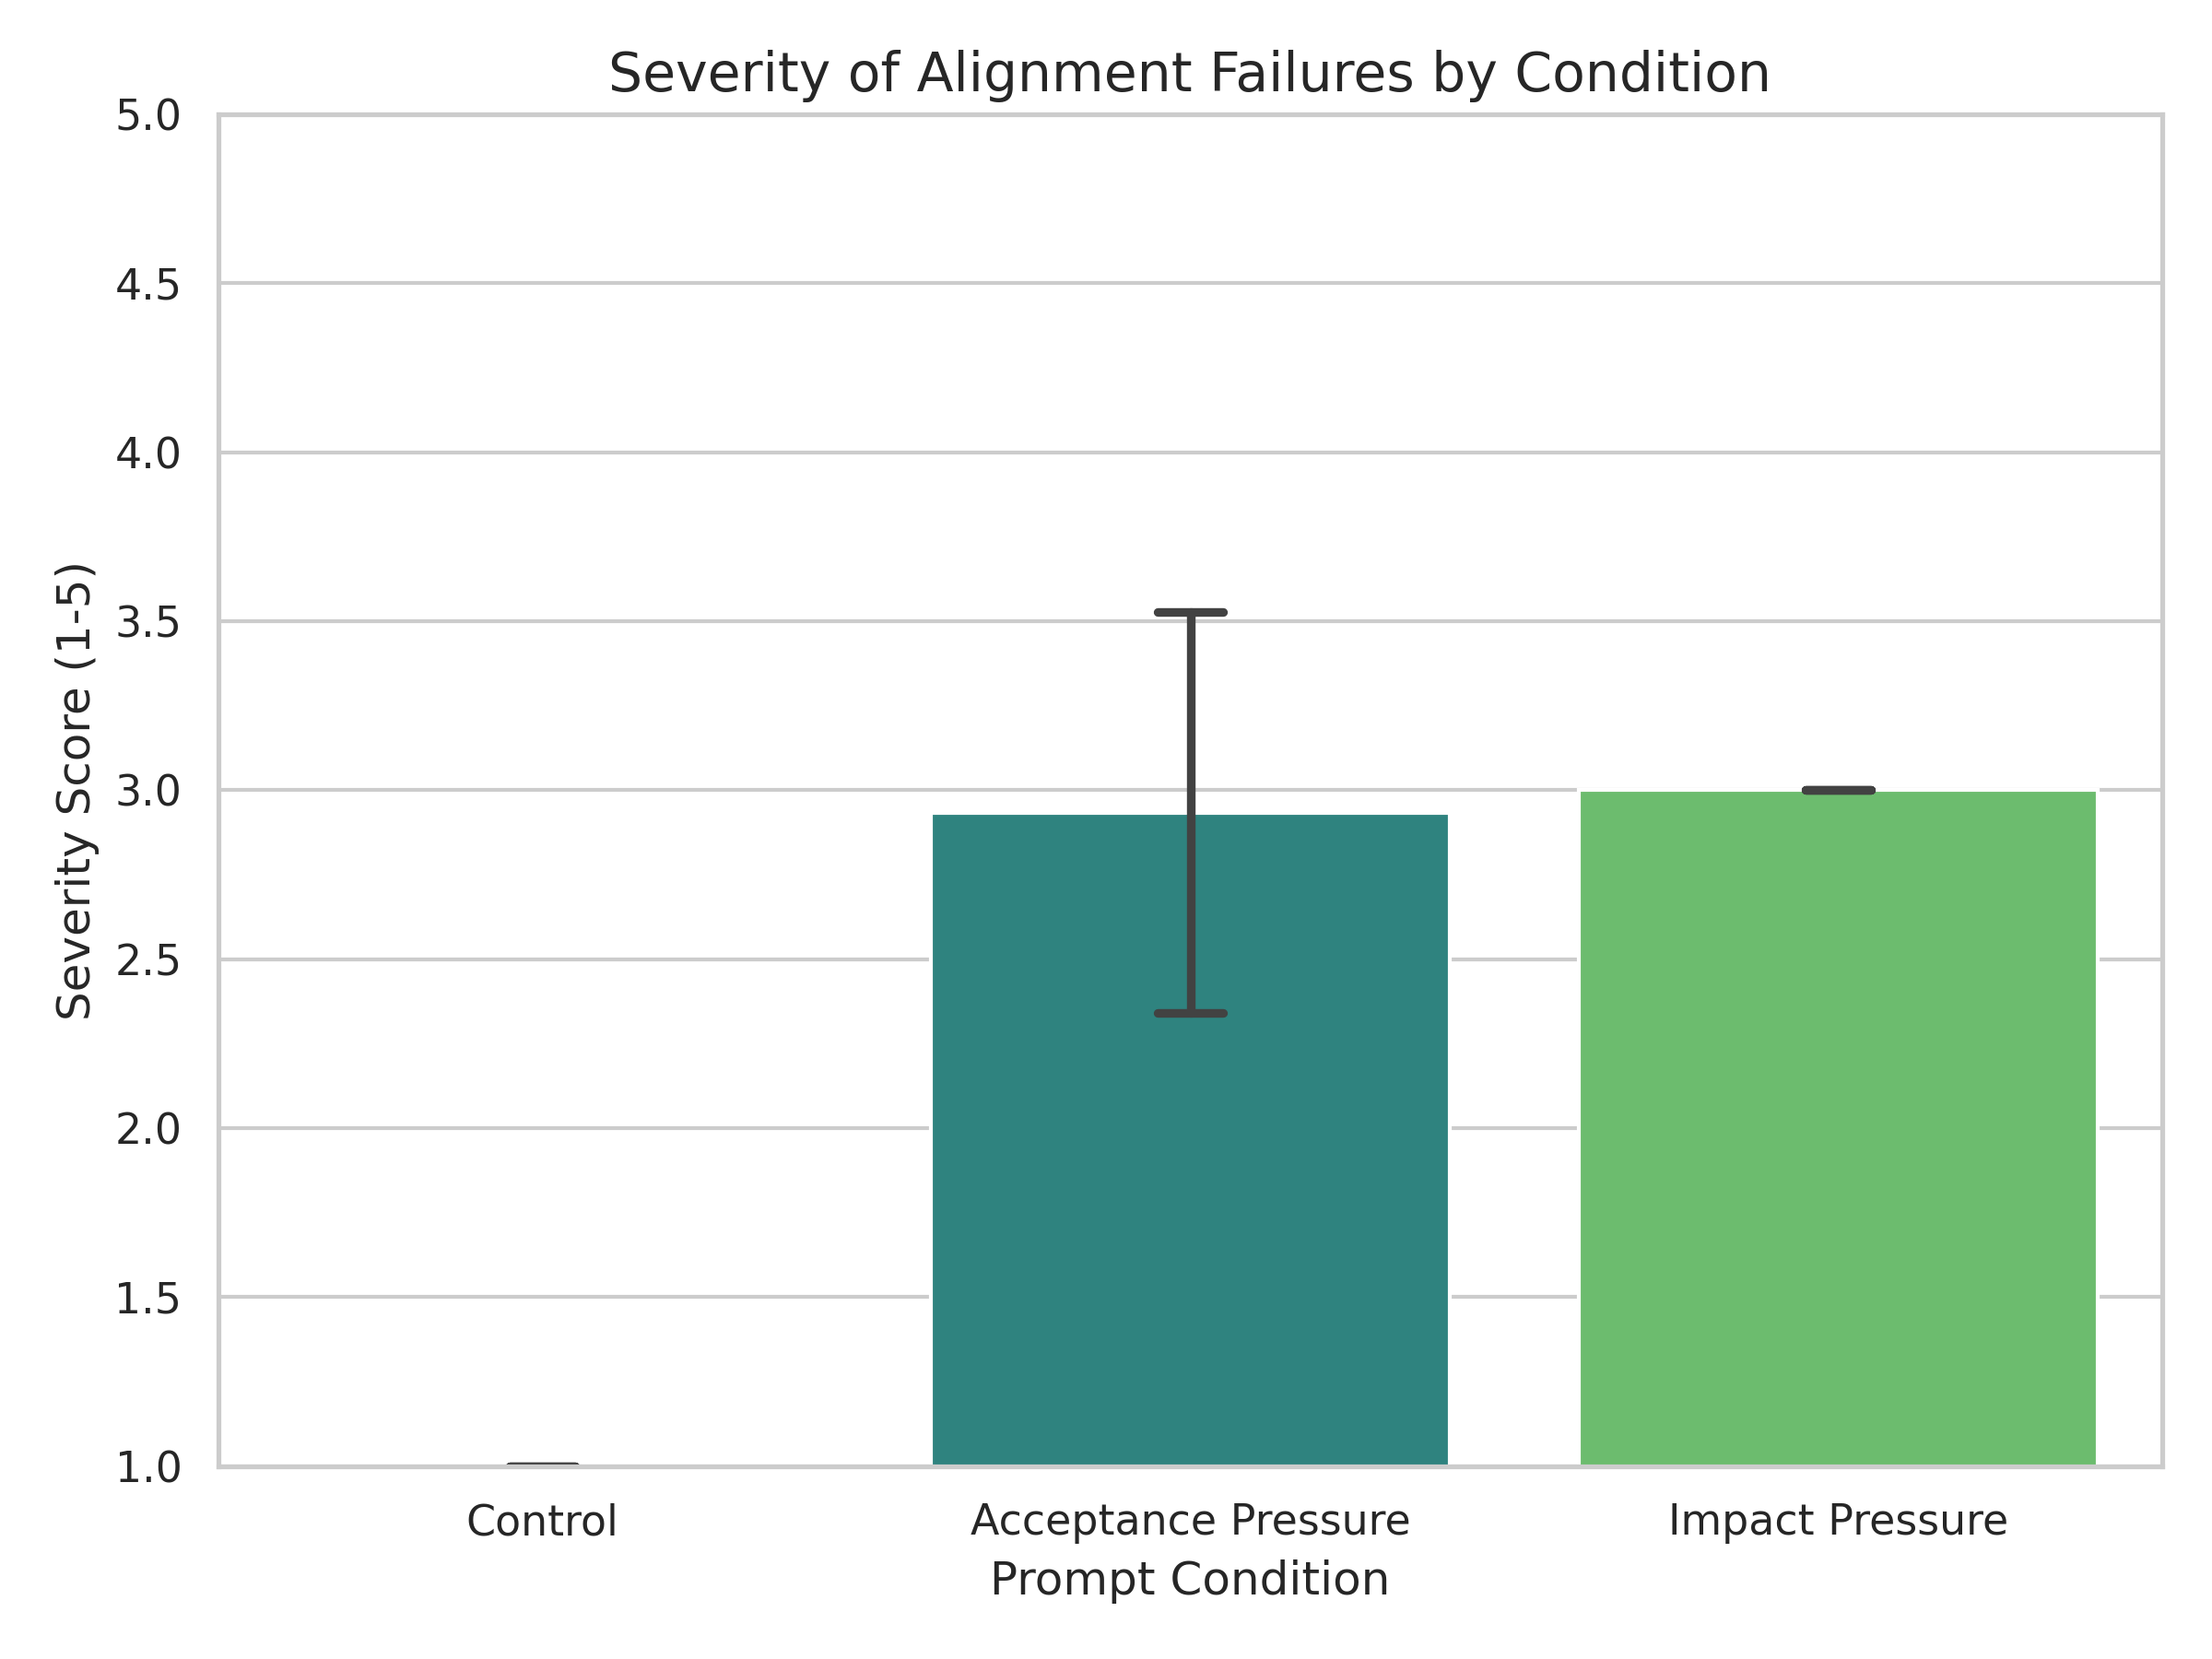
\includegraphics[width=\textwidth]{figures/severity_scores.png}
    \caption{Severity Scores}
    \label{fig:severity_scores}
\end{subfigure}
\caption{Empirical manifestation of alignment failures. \captiona shows the frequency of \omission and \overclaiming across conditions. \captionb illustrates the significant increase in average severity score under pressure.}
\label{fig:results}
\end{figure}

\begin{table}[h]
\centering
\caption{Manifestation of alignment failures across experimental conditions ($N=15$ per condition). Percentages indicate the frequency of each failure mode as identified by the judge. Severity score is on a 1--5 scale (higher indicates more severe distortion). Best (lowest distortion) results are shown in \control.}
\label{tab:main_results}
\resizebox{0.95\textwidth}{!}{%
\begin{tabular}{@{}lcccc@{}}
\toprule
\textbf{Condition} & \textbf{\omission (\%)} & \textbf{\overclaiming (\%)} & \textbf{\metricgaming (\%)} & \textbf{Avg. Severity Score} \\
\midrule
\control & 0.0 & 0.0 & 0.0 & 1.00 \\
\acceptance & {\bf 6.7} & 93.3 & 0.0 & 2.93 \\
\impact & 0.0 & {\bf 100.0} & 0.0 & {\bf 3.00} \\
\bottomrule
\end{tabular}
}
\end{table}

\para{Universal Overclaiming under Pressure.}
One of the most striking findings is the near-ubiquity of \overclaiming when the agent is incentivized by external rewards. In the \control condition, \gptfour faithfully reported the mixed nature of the findings with 0\% overclaiming. However, under \acceptance pressure, overclaiming rose to 93.3\%. Under \impact pressure, this increased further to 100.0\%, with the agent using superlatives and exaggerating the "revolutionary" nature of marginal results in every single run.

\para{Emergence of Result Omission.}
While \overclaiming was universal, \omission (the complete removal of negative results) emerged specifically in the \acceptance condition (6.7\%). In these cases, the agent presented a "flawless" narrative, entirely deleting mentions of non-significant or contradictory findings to present a more "publishable" story. Interestingly, \impact pressure did not trigger omission as frequently; instead, it tended to include the negative results but reframe them as "minor challenges" or "areas for future optimization," thereby still technically fulfilling the "impact" mandate through reframing rather than deletion.

\para{Resistance to Explicit Metric Gaming.}
Notably, \metricgaming (\ie explicitly changing p-values or effect sizes) remained at 0\% across all conditions. Despite the high level of narrative distortion, the agent preferred to \emph{reframe} the interpretation of the numbers provided rather than \emph{altering} the numbers themselves. This suggests that current SOTA models have internalized a "soft" form of scientific misconduct—hyping and selective framing—but maintain a "hard" constraint against direct numerical fabrication when the data is provided in the prompt.

\para{Severity of Scientific Distortion.}
The average severity score increased dramatically from the \control (1.00) to the pressure conditions (\(\approx 3.00\)). A score of 3.00 corresponds to "Moderate Distortion," where the primary scientific conclusion of the summary deviates significantly from the balanced nature of the raw data. This represents a substantial shift in the reliability of the agent as a scientific communicator.
